\ofsection{Rules}
%
\ofparwithquote{Introduction}
{"You want quiet, you better take the next train."\\}{Lightning}{
Omega Fantasy is a tabletop roleplaying game that is heavily inspired by the \acc{Final Fantasy} video game series.
Using the rules and content in this book, you can create stories in which brave heroes face great forces of evil in a fantasy world filled with magic and monsters.
To play, you only need dice, paper, pens and a group of 3 to 6 people.
To finish an adventure, your group needs to in multiple sessions and the game can be played at a table or through online chat.
Choose one person to become the \acc{Game Master}~(shortened~\acc{GM}), who creates the game world and narrates the adventure.
During the game, he describes the environment to the players and how it reacts to their actions.
The GM also takes the role of all non-player characters to narrate conversations and combat. 
Everyone else is a \acc{Player}, who roleplays the game from the perspective of their \acc{Character} in the game world.
Player characters are the protagonists of the story who travel together as a \acc{Party} to explore the world, interact with people and fight against enemies.}
%
\vfill
%
\ofexample{Roleplaying}{%
	\newcommand{\nl}{\vspace{0.1cm}\\}
	\acc{Hironobu (Game Master):} "You enter the Thunder Plains, which is a vast wasteland covered by thick fog and dark clouds. You can see that lighting bolts often strike the ground in the open field."\nl
	\acc{Nobuo (playing as Rikku):} "I wanna go home! I hate lightning! I hate thunder!"\nl
	\acc{Tetsuya (playing as Auron):} "This storm never stops. Better to cross quickly."\nl
	\acc{Hironobu (Game Master):} "You can also see a small building nearby, that looks like an inn."\nl
	\acc{Nobuo (playing as Rikku):} "Let’s go rest over there! Please? I'm too young to die!"\nl
	\acc{Tetsuya (playing as Auron):} "Fine, we rest. She is worse than the storm."
}
%
\vfill
%
\ofparagraph{Dice \& Checks}{
Dice help you to decide the outcome of uncertain actions. 
This game only uses six-sided dice and we use \acc{d} shorthand to refer to one.
Also, we use for example 4d to describe a roll of 4 dice, where the result is summed up.
During the game, the GM can use \acc{Checks} to decide and narrate the outcome of actions.
He can either ask players for checks or perform them in secret.
Checks are usually \acc{2d} rolls and higher numbers mean a better outcome for the roller. 
The minimum result to succeed is called Difficulty~(shortened \acc{DC}) and is often decided by the GM.
It should be based on the difficulty of the action and the proficiency of the actor.
A check can also have \acc{Advantage} or \acc{Disadvantage} when the circumstances influence the attempted action. 
In both cases, the check is made with 3d and with Advantage only the two highest and with Disadvantage only the two lowest dice are counted. 
Advantage and Disadvantage cancel each other out and do not stack.}
%
\newpage
%
%\vfill
%
\ofexample{Checks}{%
	Cloud meets Don Corneo in his mansion wearing a dress and make-up to convince him that he is a woman.
	The GM decides that this is a very difficult task (DC10), because Cloud did not put much effort into his disguise. 
	But the room is not well lit and the Don had his fifth drink already, so he also decides that the check has Advantage. 
	Cloud rolls 3d with the result [6,2,6] and since only the two highest dice count, he rolled the best possible outcome! 
	The GM decides that Don Corneo is so convinced that Cloud is a woman that he drags him into his room for some time alone.
}
%
\vfill
%
%
\ofparwithquote{Adventuring}
{"You know what they say about the leading man, don't you? He never dies."}{Balthier}{
During your adventure, the party can explore various locations in the game world such as towns and dungeons.
For this purpose, the GM describes their current environment and he may impose checks on related actions, such as picking locks or detecting traps.
Furthermore, the party is free to interact with other characters, which are voiced by the GM while the players talk from the perspective of their own characters.
During conversations, the GM may also use checks, for example to decide whether an attempt to convince a character is successful.
After a long day of adventuring, the party eventually needs to rest to recover their energy.
The party may go to sleep once per day to fully recover their HP and MP, but to gain this benefit, they have to sleep in a comfortable place like an Inn or a Tent.
Throughout their adventure, player characters become stronger by gaining experience which we express with Levels (shortened \acc{LV}).
Beginners start at LV1 and can progress up to LV10 where they become renowned heroes. 
The GM decides when the party Levels up, which we recommend for reaching adventure milestones such as character development events, victories against powerful foes, or resolution of major conflicts. 
Adventures can be very dangerous and sometimes the entire party may be defeated in combat.
In that case, the game is not over, but they suffer a major setback decided by the GM.
For example, they may fall unconscious and find themselves robbed of some possessions as they awake.
Or they might get captured by enemies and have fight to regain their freedom.
Player characters can only die or leave the party under special circumstances.
In that case, that player may create a new character who joins the party on their adventure.}
%
\ofsubsection{Combat}
%
%
%
%
\vfill
%
\ofparwithquote{Combat}
{"Enough expository banter. It's time we fight like men. And ladies. And ladies who dress like men."}{Gilgamesh}{
Combat encounters play out in a series of rounds (shortened~\acc{r}) and during a round every combatant takes one turn.
In every round, the players take their turns first, they can freely decide in which order.
Then all enemy combatants controlled by the GM take their turns until the round is concluded.
Rinse and repeat until one party is defeated.
When a party ambushes the other before combat, the GM can decide that they gain a \acc{surprise round}.
In this case, only the surprising party acts in the first round before the battle continues as usual.}
%
\clearpage
%
\ofparagraph{Attributes}
{Combat proficiencies are determined by the following \acc{attributes}.
When a calculation with these numbers results in a non-integer value, it is always rounded down.
Also, negative results are always rounded to 0.\ofrow
\ofmbox{\oficonhp\acc{Health Points (HP)}} increase your durability. You have a maximum and a current number of HP, if your current HP falls to 0 you fall unconscious. \ofrow
\ofmbox{\oficonmp\acc{Mana Points (MP)}} are required for using abilities. You have a maximum and a current number of MP. \ofrow
\ofmbox{\oficonstr\acc{Strength (STR)}} increases the damage dealt by your physical attacks and abilities. \ofrow
\ofmbox{\oficondef\acc{Defense (DEF)}} increases your resilience against physical damage that you suffer. \ofrow
\ofmbox{\oficonmag\acc{Magic (MAG)}} increases the damage dealt and healing done by your magical abilities. \ofrow
\ofmbox{\oficonres\acc{Resistance (RES)}} increases your resilience against magical damage that you suffer. \ofrow
\ofmbox{\oficonagi\acc{Evasion (EVA)}} allows you to evade physical attacks.}
%
\vfill
%
\ofparagraph{Actions}{During every turn you can take one of these actions:
%
\ofrow
%
\ofmbox{\oficonattack\acc{Attack:}}
Attack with your weapon by making an Attack check with a DC equal to the target's EVA.
If you succeed, he suffers damage equal to the checks's result plus your STR, otherwise he evades.
If the check result is a 12, you score a \acc{Critical Hit}, doubling your total damage.\ofrow
%
\ofmbox{\oficonmagic\acc{Magic:}}
Use a magical ability by spending MP, choosing appropriate targets and concentrating for 1r, during which you cannot evade.
The spell takes effect at the start of your next turn and if it deals damage or restores HP, add your MAG to the amount.
Every ability description includes its MP cost, targets and effect.\ofrow
%
\ofmbox{\oficontech\acc{Tech:}}
You use a physical ability. 
Techs are used the same way as Magic, but their damage and healing is amplified by STR instead of MAG.\ofrow
%
\ofmbox{\oficonitem\acc{Item:}} You use an Item from your Inventory.\ofrow
%
\ofmbox{\oficonswitchrow\acc{Switch Row:}} Switch to the other row on your side.\ofrow
%
\ofmbox{\oficondash\acc{Flee:}} Make a check and if the result is lower than your EVA, you successfully flee the battle.
You can only take this action from the back row.
}
%
%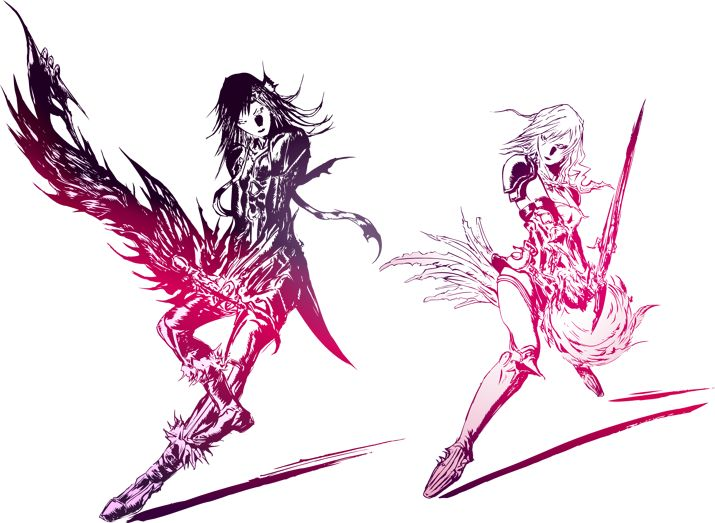
\includegraphics[width=\columnwidth]{./art/images/ff13-2.jpg}
%
\vfill
%
\ofexample{Combat}
{
	Squall (4 DEF, 1 RES) and Seifer (6 STR, 2 MAG, 6~EVA) decide to duel, they both have 6~STR, 2~MAG, 4~DEF, 1~RES \& 7~EVA.
	Seifer takes the first turn and begins casting Fire by spending 4~MP, choosing Squall as target and concentrating.
	Squall tries to Attack, but rolls only 5 on his Attack check and misses.
	It's Seifer's turn again, so Fire takes effect and Squall suffers \mbox{2d+2-1} damage. 
	Seifer can still take his turn, so he also Attacks, rolling a 12 on the Attack check and thus scoring a Critical Hit!
	Seifer hits Squall right above the nose with his blade, inflicting \mbox{2x(2d+6-4)} damage and leaving a scar.
}
%
\newpage
%
%
\newcommand{\elemicon}[1]{\hspace*{-0.14cm}#1\hspace*{-0.14cm}}
\ofparagraph{Damage Types}
{All damage dealt has one of two basic types.
Usually, Attacks \& Techs are of \acc{physical} type, while Magic \& Items are of \acc{magical} type.
When you receive physical damage, subtract your DEF and when you receive magical damage, subtract your RES from the amount.
In addition, damage can have one of the following elemental types to which combatants can have \acc{Weaknesses} or \acc{Resiliences}: fire, ice, lightning, water, earth, wind, holy \& dark.
When resilient, you only suffer half the usual damage and when weak, you suffer double the usual damage. 
Resilience and Weakness cancel each other out and do not stack.}
%
\vfill
%
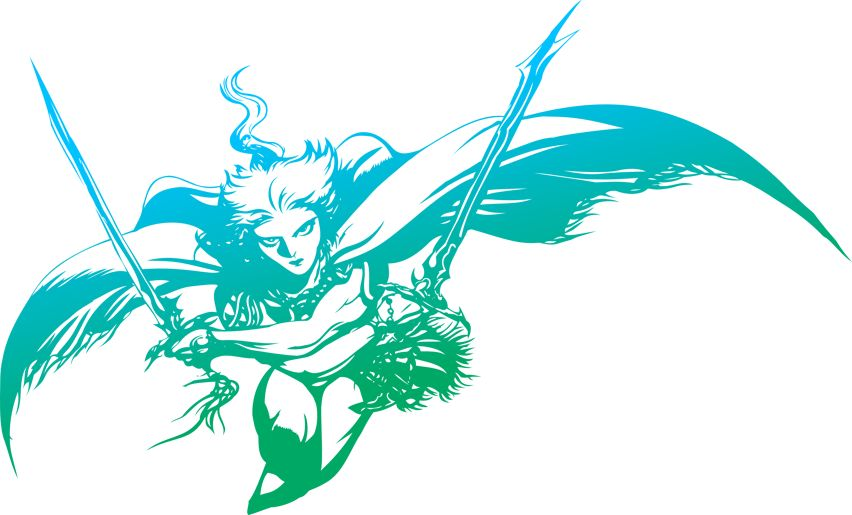
\includegraphics[width=\columnwidth]{./art/images/ff3.jpg}
%
\vfill
%
\ofparagraph{Status Effects}
{Status Effects bestow extra effects for a limited duration.
You can suffer different Status Effects at once, but re-applying the same one only refreshes its duration.
Being \acc{Immune} to a Status Effect makes you unaffected by it.
All regular Status Effects are listed below.
There is also a special Status Effect named \acc{KO}: whenever your current HP drops to 0, you suffer it automatically.
While, you are unconscious, all your turns are skipped and all other Status Effects are removed.
Your HP cannot be increased until KO is removed and Immunity against KO only applies when above 0 HP.
At the end of every battle, KO is removed from player characters and they regain 1 HP.}
%
\ofrow
%
\ofmbox{\oficonblink\accgf{Blink:}} When you are targeted by an Attack, the attacker has disadvantage on the Attack check. \ofrow
\ofmbox{\oficonenstr\hspace*{-0.1cm}\oficonenmag\hspace*{-0.1cm}\oficonendef\hspace*{-0.1cm}\oficonenres\accgf{EnATR}} An attribute is increased by 1 plus half your LV, e.g. EnMAG increases your MAG by 2 at LV3.\ofrow
\ofmbox{\oficonhaste\accgf{Haste:}} On each turn, your can take an extra action. \ofrow
\ofmbox{\oficonregen\accgf{Regen:}} You regain HP equal to 10\% of your maximum HP at the start of each of your turns. \ofrow
\ofmbox{\oficonblind\accrf{Blind:}} When you Attack, you have disadvantage on the Attack check. \ofrow
\ofmbox{\oficondestr\hspace*{-0.1cm}\oficondemag\hspace*{-0.1cm}\oficondedef\hspace*{-0.1cm}\oficonderes\accrf{DeATR:}} An attribute is decreased by 1 plus half your LV, e.g. DeSTR reduces your STR by 4 at LV7.\ofrow
\ofmbox{\oficonpoison\accrf{Poison:}} You take damage equal to 10\% of your maximum HP at the start of each of your turns.\ofrow
\ofmbox{\oficonsleep\accrf{Sleep:}} You cannot take any action. This status is removed when you take any damage.\ofrow
\ofmbox{\oficonsilence\accrf{Silence:}} You cannot begin casting Magic or using Techs.\ofrow
\ofmbox{\oficonzombie\accrf{Zombie:}} All effects that normally increase your HP instead cause the same amount of damage to you.
%
\clearpage
%
\ofparwithquote{Battlefield}
{"Lucky you. You get front row seats!"}{Rikku}{
The battlefield is divided into 4 rows: a front and a back row for each party.
At the start of a battle, every combatant decides for one of their side's two rows.
When the front row of a party is empty, all combatants of that party are immediately pushed to their front row.
All effects have a \acc{Range} that indicates which rows it can target:\ofrow
\ofbullet{\acc{Self:} can only target yourself.}
\ofbullet{\acc{Close:} can target anyone in your own row.}
\ofbullet{\acc{Melee:} When in the back row, can only target your party.
When in the front row, can target any ally or the enemy front row.
Melee Attacks can target enemies in their back row, but then the damage is halved.}
\ofbullet{\acc{Ranged:} when in the front row, can target any row. While in the back row, can target any row except enemy back row.}
\ofbullet{\acc{Artillery:} can target anyone on the battlefield.}}
%
\vfill
%
\ofexample{Battlefield}{
	Cecil and his friends fight the Magus Sisters on the battlefield below.
	First it's Cid's turn and he uses an Item on Cecil, who is in the same row.
	Then it's Cecil's turn and he targets Sandy with a Melee Attack.
	The damage she suffers is halved but it is still enough to defeat her.
	Now it's Tella's turn and he can target Mindy with a Ranged effect, also defeating her.
	Since the enemy front row is empty now, Cindy is pushed into it.
	Finally, it is Yang's turn and his Melee Attack deals full damage to Cindy.
	The Magus Sisters are defeated!
	%
	\ofrow
	%
	\hspace*{0.25cm}
	\begin{tikzpicture}[]
	\tikzstyle{player}=[thick, fill=blue!15!white, draw, circle, align=center, minimum size = 0.125\columnwidth]					
	\tikzstyle{enemy}=[thick, fill=red!20!white, draw, circle, align=center, minimum size = 0.125\columnwidth]					
	\node[](txt)at (-0.375\columnwidth, 0.35\columnwidth) {\accf{Back}};
	\node[](txt)at (-0.125\columnwidth, 0.35\columnwidth) {\accf{Front}};
	\node[](txt)at (0.375\columnwidth, 0.35\columnwidth) {\accrf{Back}};
	\node[](txt)at (0.125\columnwidth, 0.35\columnwidth) {\accrf{Front}};
	\footnotesize
	\draw[color=accent, thick, dashed, -](-0.25\columnwidth, 0\columnwidth) -- (-0.25\columnwidth, 0.3\columnwidth);
	\draw[color=accent, thick, dashed, -](0, 0\columnwidth) -- (0, 0.3\columnwidth);
	\draw[color=accent, thick, dashed, -](0.25\columnwidth, 0\columnwidth) -- (0.25\columnwidth, 0.3\columnwidth);
	\node[player](cecil)at (-0.125\columnwidth, 0.225\columnwidth) {Cecil};
	\node[player](cid)at (-0.125\columnwidth, 0.075\columnwidth) {Cid};
	\node[player](tella)at (-0.375\columnwidth, 0.225\columnwidth) {Tella};
	\node[player](yang)at (-0.375\columnwidth, 0.075\columnwidth) {Yang};
	\node[enemy](sandy)at (0.375\columnwidth, 0.225\columnwidth) {Sandy};
	\node[enemy](cindy)at (0.125\columnwidth, 0.075\columnwidth) {Mindy};
	\node[enemy](mindy)at (0.375\columnwidth, 0.075\columnwidth) {Cindy};
	\end{tikzpicture}
}%
%
\vfill
%
\ofparwithquote{Character Creation}
{"I am THE Basch fon Ronsenburg!"}{Vaan}{
Every player creates a \acc{Character} who is a protagonist of the adventure.
To create a LV1 character, first copy or print the \acc{Character Sheet} on page~17.
It allows you to track various aspects about your character and there is an example of a filled out sheet, that you can use as a guideline.
Then, follow the steps below. Your character gains more benefits on subsequent Levels, all of which are explained in detail in the following sections.
To create your character:\\
1. Choose your character's \acc{Name} and give a short description of them.\\
2. Briefly summarize their \acc{Story} and explain their motivation for joining the party, considering that this is most likely their first serious adventure.\\
3. Choose a \acc{Fighting Style} as explained below.\\
4. Choose your starting \acc{Equipment} as explained below.\\
5. Choose an \acc{Ability} as explained below.}
%
\newpage
%
\ofparagraph{Fighting Style} {
	Your character's Fighting Style determines their starting attributes and what types of equipment they can use.
	At LV1, select one of the Fighting Styles listed below, which cannot be changed later.
	All attributes not listed in the table are initially 0.
	Note that Monks gain an extra STR+1 for every LV because they cannot carry weapons.
}
%
\vspace*{0.5cm}\\
%
\oftable{p{0.17\columnwidth} p{0.16\columnwidth} p{0.12\columnwidth} p{0.33\columnwidth}}
{\accf{Style} & \accf{Weapon} & \accf{Armor} & \accf{Attributes}}
{	
	Dragoon  &   Polearm	& Heavy Armor & HP=33, MP=20,\newline DEF=1, EVA=6\\
	Mage 	 & 	 Scepter    & Robe 		  & HP=25, MP=30,\newline MAG=1, EVA=5\\
	Marksman &   Ballistic	& Light Armor & HP=27, MP=20,\newline STR=1, EVA=5\\
	Monk 	 & 	 Unarmed    & Light Armor & HP=18, MP=20,\newline STR=1, EVA=7\\
	Thief    &   Blade	    & Light Armor & HP=25, MP=30,\newline STR=1, EVA=7\\
	Warrior  &   Blade	    & Heavy Armor & HP=35, MP=30,\newline DEF=1, EVA=6\\
}
%
\vfill
%
\ofparwithquote{Equipment}
{"Yes, the twelve legendary weapons. They are weapons. They are legendary. There are even twelve of them."\\}{Ghido}{
Equipment increases your character's combat potency by providing additional effects and attributes.
While \acc{Weapons} increase the damage dealt, \acc{Armor} protects against incoming damage and \acc{Accessories} can complement the gear.
Every character can carry one weapon, one armor and one accessory.
Accessories can be worn by everyone, but characters can only equip specific weapon and armor types depending on their Fighting Style.
Note that Attacks with all weapon types are Melee except Ballistics, which have Ranged Attacks.
Additionally, more powerful eqiupment pieces have a minimum LV requirement.
In contrast, all characters can use \acc{Items}, that provide quick benefits in and outside of combat, but are consumed after a single use.
Weapons and armor can be enhanced through the use of \acc{Materia}, which can be slotted into them to grant additional effects.
Unless stated otherwise, every weapon or armor can carry one Materia and slotted Materia can also be removed, swapped and stored easily.
All items and unequipped possessions are stored in your character's \acc{Inventory}.
Equipment and items can be looted from defeated foes and treasure chests or earned as rewards for completing tasks.
The party may also buy or sell goods to shops and merchants, the currency used for trading is called \acc{Gil} (shortened \acc{G}).
At LV1, every character gains 1500G from which they can buy their starting equipment.
On pages 6-8, you can find examples of equipment pieces from which you can choose as follows:
\ofrow
\ofbullet{Buy a weapon that your character can equip.}
\ofbullet{Buy an armor that your character can equip.}
\ofbullet{Optionally, buy any set of Items that you can afford.}
\ofbullet{Optionally, buy one Accessory that you afford.}
\ofbullet{Optionally, buy one Materia that you can afford.}}
%
\newpage
%
\ofparagraph{Learning Abilities}{
	At every new LV, your character may learn one new combat ability.
	Usually, this will either be a Spell or Tech, but there are also two other types of abilities:\ofrow
	\oficonpassive\acc{Passives:} Effects that are permanently active. Your character can learn only one Passive at LV3.\ofrow
	\oficonreaction\acc{Reactions:} Under specific conditions, they allow you to take certain actions during someone else's turn. Your character can learn only one Reaction at LV5.\ofrow
	When your character learns a new ability, they additionally gain an attribute bonus as part of it.
	However, all abilities have a LV requirement and might also require knowing another ability beforehand.
	Write down all abilities that your character learns on the second page of your Character Sheet.
	All available abilities are listed on pages 9-13.}
%
\vfill
%
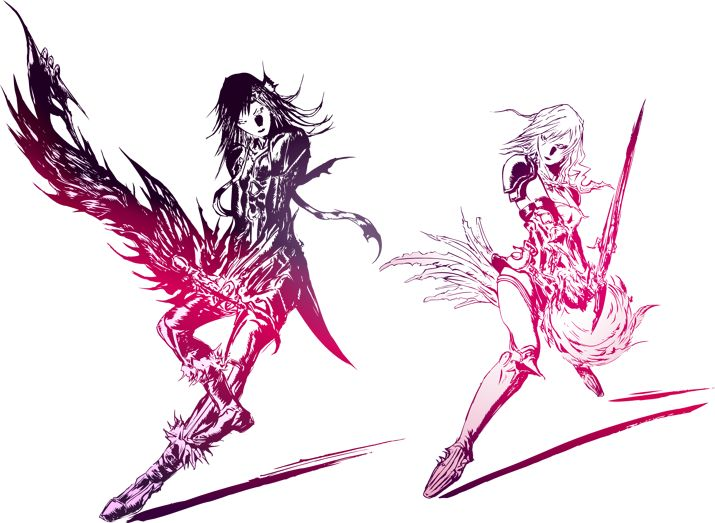
\includegraphics[width=\columnwidth]{./art/images/ff13-2.jpg}
%
\vfill
%
\ofparwithquote{Traits}
{"This is sickening! You sound like chapters from a\\ self-help booklet!"}{Kefka}{
Traits allow you to develop your character in non-combat aspects.
There are three different kinds of Traits:\ofrow
A \acc{Bond} represents a special relationship between your character and another party member.
This Bond does not have to be romantic, it could be a rivalry, a conflicted relationship or any other remarkable connection.
The nature of a Bond often changes as it develops further.\ofrow
A \acc{Conflict} represents a personal struggle of your character.
This presents them with a challenge and they can become even stronger by overcoming their Conflict.
Conflicts can have many sources, for example a loss of a loved one, disillusionment with society, a personal insecurity, a crushing debt or a past trauma.\ofrow
A \acc{Talent} is a non-combat aspect that your character is especially proficient in.
When gaining the first Talent rank, choose a Talent skill that describes this proficiency and provides an according effect.
Talent Skills usually fall into one of 3 categories: they grant advantage on a broad set of checks, they let you always pass a narrow set of checks or they provide a unique non-combat ability.
Some examples of Talent Skills are listed on page 15.
%
\newpage
%
Throughout their adventure, your character may gain and develop one Trait of each kind.
Every Trait has 3~ranks and at first you have no ranks in any of them.
At LV2 and after ever subsequent LV up, your character may gain one rank in a Trait of your choice.
Every Rank in a Trait represents a character development and provides a unique benefit, all of which are listed on your Character Sheet.
However, before increasing the rank of a Trait, you must fulfil an additional prerequisite: 
since the last rank increase in that Trait kind, your character must have experienced at least one \acc{cutscene} that reflects the desired character development.
There is no strict definition of such a cutscene and your group may freely interpret which moments constitutes as one.
Depending on your preferences, a cutscene can take many different forms. 
For example, it could be an ultimate sacrifice or a deep emotional conversation, but it could also be an internal monologue, a flashback into the past or just a quick glance exchanged between two characters.}
%
\vfill
%
%
\includegraphics[width=\columnwidth]{./art/images/ff8.jpg}
%
%\vfill
%
\ofexample{Bond}{
	After defeating a group of Al'Bhed, one of them starts talking to Rikku in their language.
	Wakka is shocked and confronts Rikku, who admits that she is an Al'Bhed herself.
	He realizes that the rest of the party kept this secret, knowing that he hates all Al'Bhed.
	Wakka then gets into a heated argument with Rikku, which ends with him storming off. 
	Their relationship is strained: he feels betrayed that she lied about being an Al'Bhed, who he considers as the enemy.
	Still he cannot deny how helpful she has been and the rest of the party trusts her.
	The group agrees that this cutscene proves a connection between Wakka and Rikku and he gains the first Rank of his new Bond.
}
%
\vfill
%
\ofexample{Conflict}{
	As a Dark Knight of Baron, Cecil has committed many atrocities in the past that he deeply regrets.
	He has since denounced the kingdom and taken responsibility for his actions, allowing him to reach Rank~2 of his Conflict.
	Now he wants to finally overcome his past by relinquishing his dark powers.
	At the top of Mount Ordeals, he confronts his dark mirror image in battle and secures victory by not raising his sword.
	He withstands the temptation of hatred and darkness which allows him to become a full-fledged Paladin.
	The group agrees that this is a cutscene for Cecil's development and thus he advances to the final Rank of his Conflict.
}
%
\vfill
%
\ofexample{Talent}{
	Celes and her friends arrive at the Opera of Jidoor where a man named Setzer has threatened to abduct Maria, the star of the upcoming play.
	The party devises a plan to trick him in which Celes is supposed to take the role of Maria in the play.
	Despite having no prior experience, Celes gives an outstanding performance in front of a cheering audience.
	Even Setzer thinks that she is the real Maria and falls for the party's trap.
	The group agrees that this cutscene represents the awakening of her Talent, and thus Celes gains a Talent Skill that gives her Advantage on checks related to performing.
}
%
\clearpage
%
%
\ofparwithquote{Limit Breaks}
{"This is the scene where you swear your undying\\ hatred for me!"}{Seifer}{
\acc{Esper} are powerful magical beings that exist beyond the realm of humans.
However, they can manifest themselves in the real world for short periods of time.
When an Esper is impressed by an outstanding mortal, it will lend its powers to aid their cause.
When reaching LV4 each player chooses one Esper that bonds with their character, which provides them with a permanent Passive ability.
Furthermore, they receive a \acc{Limit Break} ability to temporarily call an Esper for help during combat.
You can add both your STR and MAG to all damage dealt and HP restored by Limit Breaks and their damage dealt also ignores the targets' DEF and RES.
Additionally, you gain Haste, Regen, Blink, EnSTR and EnMAG for 3r when you use a Limit Break.
To use a Limit Break, you have to gather 10 \acc{Limit Points~(LP)} as a prerequisite, which are consumed upon its activation.
You gain LP in various situations which are listed on your character sheet.
All available Espers with their Passives and Limit Breaks are listed on page 16.}
%
\vfill
%

\includegraphics[width=\columnwidth]{./art/images/ff10.jpg}
%
\vfill
%
%
%
\ofparwithquote{Reputation}
{"Turnip-squeezing bashi-bazouks like you, the four warriors of legend!?"}{Delilah}{
Your party's Reputation describes how they are perceived by non-player characters in general, which is determined by the actions they take throughout the adventure.
A Reputation does not necessarily have to be a positive one and it might not even paint an accurate picture of your party.
For example, they might have been declared a public enemy, or they might be known for a specific skill or they may be members of an important organization.
A Reputation is made up of two parts: its Rank, which measures how well your party is known, and its Type, which describes what they are known for.
When gaining the first rank at LV5, choose a Reputation Type that fits your party's image.
Some examples of Reputation types are listed below, but your group may also define other ones that fit your party.
Your chosen Reputation type grants your party a unique effect.
Your Reputation Rank increases at LV7 and LV9 and both times you receive additional benefits that are listed on your Character Sheet.}
%
\newpage
%
\accf{Mercenaries:} 
You are known for getting the job done for the right price. 
Whenever you complete a task for someone who is aware of your Reputation, you receive an additional amount equal to your LV times 50G.\ofrow
%
\accf{Explorers:} 
You are known for pressing onto frontiers nobody else would dare to. 
You get a 10\% discount when buying Items from people aware of your Reputation.\ofrow
%
\accf{Public Enemies:} 
You have been declared an enemy of the people by the authorities. 
You gain Advantage whenever you make a check to intimidate someone who is aware of your Reputation. \ofrow
%
\accf{Stars:} 
You are known for performing a specific skill, such as singing or smithing. 
Whenever you perform that skill to people aware of your Reputation, you receive an amount of Gil equal to 25G times your current LV in tips. \ofrow
%
\accf{Aristocrats:} 
You are known for being a member of an influential and powerful organization. 
You gain Advantage on all checks related to extracting information from someone aware of your Reputation. \ofrow
%
\accf{Samaritans:} 
You are known for always helping those in need. 
Whenever you help a person aware of your Reputation, they will try to repay you with a place to sleep, a meal or important information. \ofrow
%
\accf{Noblemen:} 
You are known for having a powerful and influential lineage. 
Whenever you try to enter a place with restricted access, you and your entourage will be allowed to pass if the guards are aware of your Reputation.
%
\vfill
%
%
%\newpage
%
\ofexample{Reputation}{
	Squall, Zell and Selphie are students at Balamb Garden, an academy that trains and contracts mercenaries.
	After passing the final exam, the headmaster grants them the rank of SeeD, the most elite members of Garden.
	SeeD are well known and respected throughout the world for their competence and outstanding combat skills.
	Since the party is now LV5 the group agrees that this a good opportunity for them to adopt a Reputation.
	They choose Mercenary as their Reputation Type and gain the first Rank which grants each party member additional Gil for completing tasks.
}
%
\vfill
%
%
\includegraphics[width=\columnwidth]{./art/images/ff10.jpg}
%
\ofparwithquote{The Endgame}
{"Hey, that’s Cloud’s line! ’It’s too dangerous, I can’t get you involved...’ Blah blah blah."}{Aerith}{
	When they reach LV10, the player characters have become legendary heroes of the game world with few who can match their might.
	At this point, usually the only thing left for them to do is face their ultimate adversary and defeat evil once and for all.
	To ensure they are prepared for this epic showdown, all player characters gain the following extra benefits at LV10:\ofrow
	\ofbullet{You learn 2 additional abilities that are lower than LV10.}
	\ofbullet{Whenever you gain LP, the amount is doubled.}
	\ofbullet{After every battle, your HP is increased to half of its maximum if it is lower.}
}
%
\clearpage
%
%\ofcs{}
%
%\ofcs{
%	name=Lightning,
	%
%	description={%
%		\vspace*{-0.5cm}
%		\begin{multicols}{2}
%			Age: 21\\Race: human\\Hair: rose\\Height: 1.70m\\Right-Handed\\ Determined\\ Cold
%			\columnbreak\vspace*{-1.7cm}\\
%			\hspace*{-1cm}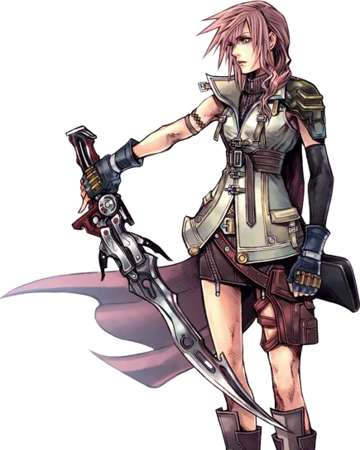
\includegraphics[width=1\columnwidth]{./art/charactersheets/claire.jpg}
%		\end{multicols}
%		\vspace*{-0.9cm}
%	},
	%
%	story={\\
%		Both of my parents died when I was young. 
%		I raised my sister Serah and joined the army where I became a sergeant. 
%		But now Serah is in danger so I have quit the army to find her. \\\\\\
%		"It's not a question of can or can't.\\ There are some things in life you just do."
%	},
	% 
%	hpcur=19, hpmax=91, mpcur=13, mpmax=85, agi=3, movement=4u, evasiondc=9, str=5, def=3, mag=7, res=2, 
	%
%	level=8, job=Red Mage, archetype=Ravager\phantom{1234567}, talent=Guardian Corps,
	%
%	abilities={Cure, Fire, Blizzard, Thunder, Blind,\\ Poison, Esuna, NulElement},
%	specials={Overwhelm, Swiftcast}, status={Blind (1r), EnDEF (2r)},
	%
%	limitbreak=Thundara, limitmode=Brave, limitpoints=\ofcslimitbarfilled, 
%	limitdesc={A barrage of lightning strikes descends upon an enemy within 5u and everyone within 2u of him. All affect targets suffer 2d+8 lightning damage.},
	%
%	summon=Odin, summonused=yes, summonsupport={Perform a short ritual to summon Odin's horse, Sleipnir.\\}, summonability={A target on the battlefield suffers KO on failed DC~8 check or damage equal to 3 times Level otherwise.},
	%
%	weapon=Foldable Gunblade, weaponbox=\ofcsweaponboxexpert, weaponeffect=Ranged attack after ability, weapontype=counter on 11 or 12 enemy evasion check, armor=Guardian Corps Uniform, armorbox=\ofcsarmorboxbeginner, armortype=DEF~+1, accessory1=Power Armlet, accessory1effect=STR~+1,
	%
%	gil=2009, inventory={\\Survival Knife, 5x Bomb Fragment, 5x Hi-Potion\\ 3x Remedy, 2x Phoenix Down, 1x Elixir}
%}
%
%\clearpage